% БҮЛЭГ 4 — ӨГӨГДЛИЙН БОЛОВСРУУЛАЛТ
% Эх: diploma_0.2v.docx, БҮЛЭГ 4. ӨГӨГДЛИЙН БЭЛТГЭЛ

\chapter{Өгөгдлийн боловсруулалт}
\label{Chapter4}

%-------------------------------------------------------------------------------
\section{Өгөгдлийн цуглуулалт}

Системийн өгөгдлийн багц нь \textbf{найман} нийтэд нээлттэй эх сурвалжаас бүрдэнэ
(Хүснэгт~\ref{tab:data_full_corpus}): news.mn (42.3\%), gogo.mn (28.1\%),
IKON.mn (9.2\%), E-Mongolia (6.4\%), ``Мэдэхгүй зүйлээ асуу'' (6.3\%),
Medee.mn (3.4\%), Zaluusinfo (2.3\%), Eagle News (1.9\%).
Олон эх сурвалжаас өгөгдөл цуглуулсан нь судалгааны салбарын олон талт байдлыг (domain diversity) хангахад чухал үүрэгтэй.

\textbf{Кирилл шүүлт.} Нийт тэмдэгтийн 85-аас дээш хувь нь кирилл бус тэмдэгтээс бүрдсэн тохиолдолд тухайн өгөгдлийг хасна. Латин үсгээр бичсэн, холимог хэлтэй болон "байна" (bn), "зүгээр" (zgr) гэх мэт албан бус товчилсон бичлэгийн хэлбэрүүдийг MN-BERT токенчлогчийн үр ашгийг хадгалах зорилгоор өгөгдлийн багцаас хасав.

Цуглуулалтыг web scraping (мэдээний сайтууд) болон нийтийн Graph API
(Facebook)-ээр хэрэгжүүлж, 2025--2026 оны нийтлэлүүдийг stratified sampling-аар цуглуулсан.

Шошголсон 10,000 дээжийн ангиллын бүтцийг Хүснэгт~\ref{tab:collection}-д,
эх сурвалжийн тархалтыг Хүснэгт~\ref{tab:data_full_corpus}-д нэгтгэсэн бол
харааны шинжилгээг Зураг~\ref{fig:data_analysis_combined}-д харуулав.

\begin{table}[H]
\centering
\caption{Ангилал тус бүрийн шошгологдсон сэтгэгдлийн тоо (n=10{,}000;
  эх сурвалжийн задаргааг Хүснэгт~\ref{tab:data_full_corpus}-аас үзнэ үү)}
\label{tab:collection}
\begin{tabular}{@{}lcc@{}}
\toprule
\textbf{Ангилал} & \textbf{Нийт сэтгэгдэл} & \textbf{Хувь (\%)} \\
\midrule
Бүтээлч шүүмжлэл  & $4{,}356$ & $43.56\%$ \\
Саармаг           & $3{,}026$ & $30.26\%$ \\
Хортой сөрөг      & $1{,}963$ & $19.63\%$ \\
Эерэг             & $655$     & $6.55\%$  \\
\midrule
\textbf{Нийт}   & $\mathbf{10{,}000}$ & $\mathbf{100\%}$ \\
\bottomrule
\end{tabular}
\end{table}

% ── Шошголсон өгөгдлийн эх сурвалжийн хүснэгт (10k) ────────────────────────
\begin{table}[H]
\centering
\caption{Шошголсон өгөгдлийн эх сурвалжийн тархалт (n=10{,}000)}
\label{tab:data_full_corpus}
\begin{tabular}{@{}lcc@{}}
\toprule
\textbf{Эх сурвалж} & \textbf{Тоо} & \textbf{Хувь (\%)} \\
\midrule
news.mn                & $4{,}230$ & $42.3\%$ \\
gogo.mn                & $2{,}811$ & $28.1\%$ \\
IKON.mn                & $919$     & $9.2\%$  \\
E-Mongolia             & $644$     & $6.4\%$  \\
Мэдэхгүй зүйлээ асуу  & $632$     & $6.3\%$  \\
Medee.mn               & $342$     & $3.4\%$  \\
Zaluusinfo             & $234$     & $2.3\%$  \\
Eagle News             & $188$     & $1.9\%$  \\
\midrule
\textbf{Нийт} & $\mathbf{10{,}000}$ & $\mathbf{100\%}$ \\
\bottomrule
\end{tabular}
\end{table}

Эх сурвалж тус бүрийн ангиллын задаргааг (аль өгөгдөл аль ангилалд хамаарсан)
Хүснэгт~\ref{tab:source-category}-д үзүүлэв.

\begin{table}[H]
\centering
\caption{Эх сурвалж $\times$ ангиллын задаргаа (n=10{,}000)}
\label{tab:source-category}
\fittable{%
\begin{tabular}{@{}lccccc@{}}
\toprule
\textbf{Эх сурвалж} & \textbf{Бүтээлч} & \textbf{Саармаг} & \textbf{Эерэг} & \textbf{Хортой} & \textbf{Нийт} \\
\midrule
news.mn               & $2{,}050$ & $920$ & $239$ & $1{,}021$ & $4{,}230$ \\
gogo.mn               & $1{,}417$ & $623$ & $191$ & $580$ & $2{,}811$ \\
IKON.mn               & $313$ & $371$ & $59$ & $176$ & $919$ \\
E-Mongolia            & $296$ & $315$ & $33$ & $0$ & $644$ \\
Мэдэхгүй зүйлээ асуу & $37$ & $523$ & $40$ & $32$ & $632$ \\
Medee.mn              & $123$ & $112$ & $29$ & $78$ & $342$ \\
Zaluusinfo            & $35$ & $106$ & $54$ & $39$ & $234$ \\
Eagle News            & $85$ & $56$ & $10$ & $37$ & $188$ \\
\midrule
\textbf{Нийт} & $\mathbf{4{,}356}$ & $\mathbf{3{,}026}$ & $\mathbf{655}$ & $\mathbf{1{,}963}$ & $\mathbf{10{,}000}$ \\
\bottomrule
\end{tabular}}
\end{table}

% ── Харааны шинжилгээний зураг ───────────────────────────────────────────────
\begin{figure}[H]
  \centering
  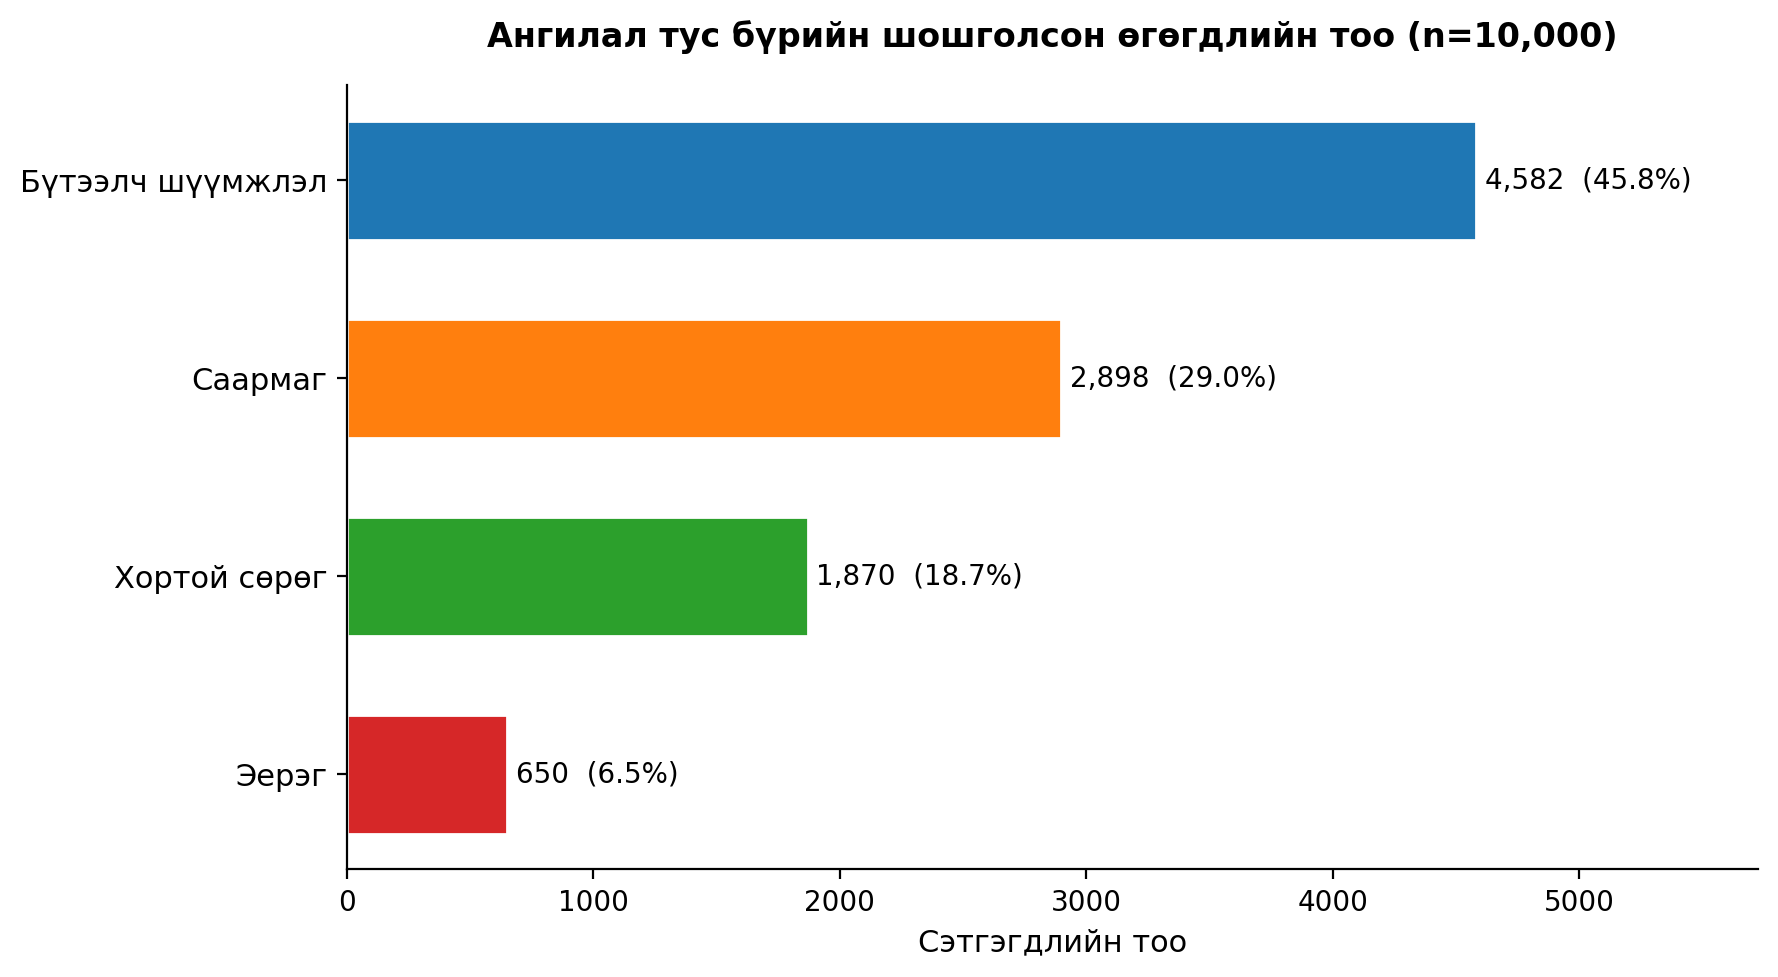
\includegraphics[width=0.78\textwidth]{Figures/data_categories_bar.png}
  \caption{Шошголсон 10,000 дээжийн ангиллын тархалт. Бүтээлч шүүмжлэл ангилал
    (43.56\%) тодорхой давамгайлж байна.}
  \label{fig:data_analysis_combined}
\end{figure}

Ангиллын харьцаа 6.6:1 байгаа нь өгөгдлийн багц дахь ангиллын тархалт илт тэнцвэргүй байгааг харуулж байна. Суурь загваруудад SMOTE,
MN-BERT-д Focal Loss ($\gamma{=}2.0$) + WeightedRandomSampler-ийг хэрэглэсэн
(бүлэг~\ref{Chapter5}).

%-------------------------------------------------------------------------------
\section{Өгөгдлийн цэвэрлэгээ ба урьдчилсан боловсруулалт}

Цуглуулсан хам текстийг дараах дамжлагаар боловсруулна:

\textbf{Кирилл шүүлт.} Нийт тэмдэгтийн 85-аас дээш хувь нь кирилл бус тэмдэгтээс бүрдсэн тохиолдолд тухайн өгөгдлийг хасна (тоо, цэг таслал зөвшөөрнө). MN-BERT-ийн vocabulary кирилл корпус дээр суурилсан тул токенчлолоос өмнө явагдана.

\textbf{Текст нормчлол.} HTML/URL хасч, эможийг \texttt{[EMOJI]} орлуулагчид хөрвүүлнэ: MN-BERT-ийн SentencePiece токенчлогч нь кирилл корпус дээр сургагдсан тул эможийг толь бичигт байхгүй (OOV) дэд үгэн хэсгүүдэд хувааж, урьдчилан сургасан дүрслэлийн тогтвортой байдлыг алдагдуулдаг. Тиймээс \texttt{[EMOJI]} орлуулга нь архитектурын зайлшгүй шаардлага болно.

\textbf{Токенчлол.} MN-BERT: нормчлол $\to$ SentencePiece токенчлол (стоп үг хасах, stemming \emph{хийхгүй}; залгамал (agglutinative) морфологийг дотооддоо задалдаг).
Суурь загварт (LR, NB, SVM): нормчлол $\to$ TF-IDF $\to$ стоп үг хасах.

%-------------------------------------------------------------------------------
\section{Шошгологдолтын стратеги}

Шошгологдолт нь дөрвөн ангилалыг хамарна: \textbf{Эерэг}, \textbf{Саармаг},
\textbf{Хортой сөрөг} (хувь хүнд чиглэсэн доромжлол/дарамт),
\textbf{Бүтээлч шүүмжлэл} (аргументтай, шийдэл санал агуулсан сөрөг хандлага).
Монгол хэлийг эх хэл болгон ярьдаг, Монголын цахим орчны хэлэлцүүлэгтэй танил 3 шошгологч нарийн зааврын дагуу ажилласан.

Шошгологдолтыг дараах 3 алхамаар зохион байгуулсан:

\begin{enumerate}
  \item \textbf{Зааврын боловсруулалт.} Ангилал тус бүрийн тодорхойлолт, хилийн
    тохиолдлын жишээ, Егөөдөл (irony) таних зарчим болон бусад зааврыг агуулсан бичгийн удирдамж бэлтгэв.
  \item \textbf{Бие даасан шошгологдолт.} 3 шошгологч хамааралгүйгээр бүх 10,000 дээжийг шошголов.
  \item \textbf{Нийцлийн хэмжилт.} Fleiss' $\kappa$-аар нийцлийг тооцоолж, зөрөлдөөнийг хэлэлцэлтээр шийдэв.
\end{enumerate}

\textbf{Аннотацийн заавар:} кирилл текст авах, тодорхойгүй тохиолдолд ``ambiguous'' тэмдэглэх. \textbf{Хил хязгаарын гол дүрэм:} нийгмийн тогтолцоо, байгууллага, бодлогод чиглэсэн шүүмжлэлийг хэчнээн хурц хэлтэй байсан ч \textbf{Бүтээлч шүүмжлэл}д шошголно (методологийн үндэслэл: тогтолцоо руу чиглэсэн шүүмжлэл нь хувь хүнд чиглэсэн халдлага биш; ``хортой'' гэж тэмдэглэх нь хэрэглэгчийн үзэл бодлоо илэрхийлэх эрхийг зөрчинэ). Эцсийн Fleiss' $\kappa{=}0.72$ (хангалттай нийцэл); зөрөлдөөнийг консенсусаар шийдвэрлэв. Үйл явцыг Зураг~\ref{fig:annotation-process}-д харуулав.

\begin{figure}[H]
\centering
\begin{tikzpicture}[
  mainbox/.style={draw, rounded corners=5pt, minimum width=5.5cm,
                  minimum height=1.20cm, text width=5.1cm,
                  align=center, font=\small, line width=0.8pt},
  annotbox/.style={draw, rounded corners=5pt, minimum width=2.8cm,
                   minimum height=1.20cm, text width=2.5cm,
                   align=center, font=\small, line width=0.8pt},
  decbox/.style={diamond, draw, aspect=2.8, minimum width=3.8cm,
                 inner sep=2pt, align=center, font=\small, line width=0.8pt},
  arr/.style={->, >=Stealth, thick, line width=0.9pt},
]

% ── INPUT ────────────────────────────────────────────────────────────────
\node[mainbox, fill=gray!12, draw=gray!50] (inp) at (0, 0)
  {\textbf{Хам сэтгэгдэл}\\[1pt]
   {\scriptsize $n = 10{,}000$ · найман эх сурвалж}};

% ── ANNOTATION GUIDELINES ────────────────────────────────────────────────
% gap: 2.20 - 0.60 - 0.60 = 1.00 cm
\node[mainbox, fill=blue!10, draw=blue!45] (guide) at (0,-2.20)
  {\textbf{Аннотацийн заавар}\\[1pt]
   {\scriptsize Хил хязгаар · ирони · дүйцэшгүй тохиолдол}};

% ── 3 ANNOTATORS (side by side) ──────────────────────────────────────────
% vertical gap from guide.south(-2.80) to a2.north(-3.80) = 1.00 cm
\node[annotbox, fill=orange!14, draw=orange!55] (a1) at (-3.5,-4.40)
  {\textbf{Шошгологч 1}\\[1pt]
   {\scriptsize Бие даан\\шошголоно}};
\node[annotbox, fill=orange!14, draw=orange!55] (a2) at (0,-4.40)
  {\textbf{Шошгологч 2}\\[1pt]
   {\scriptsize Бие даан\\шошголоно}};
\node[annotbox, fill=orange!14, draw=orange!55] (a3) at (3.5,-4.40)
  {\textbf{Шошгологч 3}\\[1pt]
   {\scriptsize Бие даан\\шошголоно}};

% ── KAPPA MEASUREMENT ────────────────────────────────────────────────────
% gap: 6.60 - 4.40 - 0.60 - 0.60 = 1.00 cm
\node[mainbox, fill=yellow!18, draw=yellow!70!black] (kappa) at (0,-6.60)
  {\textbf{Нийцлийн хэмжилт}\\[1pt]
   {\scriptsize Fleiss' $\kappa = 0.72$ · хангалттай нийцэл}};

% ── DISAGREEMENT DECISION ────────────────────────────────────────────────
% kappa.south=-7.20; dec.north=-8.22 → gap=1.02 cm
\node[decbox, fill=yellow!20, draw=yellow!70!black] (dec) at (0,-8.90)
  {Зөрөлдөөн?};

% ── CONSENSUS (right of diamond) ─────────────────────────────────────────
% dec.east=1.90; cons.west=5.80-2.75=3.05 → gap=1.15 cm
\node[mainbox, fill=red!8, draw=red!40] (cons) at (5.80,-8.90)
  {\textbf{Консенсус хэлэлцэх}\\[1pt]
   {\scriptsize Зөрөлдсөн дээжийг\\3 шошгологч ярилцана}};

% ── FINAL LABEL ──────────────────────────────────────────────────────────
% dec.south=-9.58; final.north=-10.53 → gap=0.95 cm
\node[mainbox, fill=green!14, draw=green!55] (final) at (0,-11.13)
  {\textbf{Эцсийн шошго}\\[1pt]
   {\scriptsize Эерэг · Саармаг · Хортой сөрөг · Бүтээлч шүүмжлэл}};

% ── OUTPUT DATASET ───────────────────────────────────────────────────────
% gap: 13.33 - 11.13 - 0.60 - 0.60 = 1.00 cm
\node[mainbox, fill=blue!14, draw=blue!50] (out) at (0,-13.33)
  {\textbf{Шошгологдсон датасет}\\[1pt]
   {\scriptsize $n = 10{,}000$ · 4 ангилал · сургалтад бэлэн}};

% ── ARROWS ───────────────────────────────────────────────────────────────
\draw[arr] (inp)   -- (guide);
\draw[arr] (guide) -- (a1);
\draw[arr] (guide) -- (a2);
\draw[arr] (guide) -- (a3);
\draw[arr] (a1)    -- (kappa);
\draw[arr] (a2)    -- (kappa);
\draw[arr] (a3)    -- (kappa);
\draw[arr] (kappa) -- (dec);

% Тийм (there is disagreement) → consensus
\draw[arr] (dec.east) -- node[above, font=\scriptsize] {Тийм} (cons.west);

% Үгүй (all agree) → final label directly
\draw[arr] (dec.south) -- node[right, font=\scriptsize, xshift=2pt] {Үгүй} (final.north);

% Consensus → final (L-shaped: down then left)
\draw[arr] (cons.south) |- (final.east);

\draw[arr] (final) -- (out);

\end{tikzpicture}
\caption{Аннотацийн үйл явцын диаграмм: хам сэтгэгдлийг тодорхой зааврын
  дагуу 3 бие даасан шошгологч шошголж, Fleiss' $\kappa$-ийн хэмжилтээр
  нийцлийг баталгаажуулж, зөрөлдсөн дээжийг консенсусаар шийдэн
  шошгологдсон датасет бүрдүүлнэ.}
\label{fig:annotation-process}
\end{figure}

Шошгологдолтын дараа ангиллуудын тоон тэнцвэрийг шалгаж, тэнцвэржүүлэлтийг
суурь загваруудад SMOTE-оор, эцсийн нэг шатлалт MN-BERT загварт ангиллын жин
оногдуулсан Focal Loss ($\gamma=2.0$) болон WeightedRandomSampler-аар
хэрэгжүүлнэ (дэлгэрэнгүйг бүлэг~\ref{Chapter5}).

%-------------------------------------------------------------------------------
\section{Өгөгдлийн хайгуулын шинжилгээ (EDA)}

Загвар сургалтын өмнө 10,000 дээжийн хайгуулын шинжилгээ (EDA) хийж өгөгдлийн
бүтцийг тодорхойлов.

\textbf{Ангиллын тархалт.} Бүтээлч 43.56\%, Саармаг 30.26\%, Хортой сөрөг 19.63\%,
Эерэг 6.55\% (Хүснэгт~\ref{tab:collection}, Зураг~\ref{fig:data_analysis_combined}) ---
Монгол сошиал медиад шүүмжлэх хандлага давамгайлж байна.

\textbf{Сэтгэгдлийн урт.} Медиан урт (Зураг~\ref{fig:len-dist}): Бүтээлч шүүмжлэл
$\approx 137$, Хортой сөрөг $\approx 93$, Эерэг $\approx 90$, Саармаг $\approx 59$ тэмдэгт.

\begin{figure}[H]
\centering
\begin{tikzpicture}
\begin{axis}[
  xbar,
  width=10cm, height=5.5cm,
  bar width=0.5cm,
  xlabel={Сэтгэгдлийн медиан урт (тэмдэгт)},
  ytick={1,2,3,4},
  yticklabels={Хортой сөрөг, Саармаг, Эерэг, {Бүтээлч шүүмжлэл}},
  xmin=0, xmax=185,
  nodes near coords,
  nodes near coords align={horizontal},
  every node near coord/.style={font=\small},
  enlarge y limits=0.25,
  tick label style={font=\small},
  label style={font=\small},
]
\addplot[fill=blue!40] coordinates {
  (93,1)
  (59,2)
  (90,3)
  (137,4)
};
\end{axis}
\end{tikzpicture}
\caption{Ангилал тус бүрийн сэтгэгдлийн медиан урт (тэмдэгтийн тоо)}
\label{fig:len-dist}
\end{figure}

\textbf{N-gram шинжилгээ.} Хортой сөрөг-д доромжлол/халдлага, Бүтээлч
шүүмжлэлд ``засах''/``хэрэгтэй'' зэрэг үгс давамгайлна; давхцлыг
Зураг~\ref{fig:euler-vocab}-д үзүүлсэн.

\begin{figure}[H]
\centering
\begin{tikzpicture}[font=\small]

% Two equal circles: r=2.7cm, centers at (-2.0,0) and (2.0,0)
% center distance=4.0cm → overlap region x∈[-0.7, +0.7]

\draw[fill=red!30, fill opacity=0.55, draw=red!70, line width=1.5pt]
  (-2.0, 0) circle (2.7cm);
\draw[fill=blue!28, fill opacity=0.55, draw=blue!68, line width=1.5pt]
  ( 2.0, 0) circle (2.7cm);

% ── TITLES ───────────────────────────────────────────────────────────────
\node[font=\normalsize\bfseries, text=red!75!black]
  at (-2.0, 3.15) {Хортой сөрөг};
\node[font=\normalsize\bfseries, text=blue!75!black]
  at ( 2.0, 3.15) {Бүтээлч шүүмжлэл};

% ── OVERLAP HEADER (x=0: both dists=2.0<2.7 ✓) ──────────────────────────
\node[font=\footnotesize\bfseries, text=gray!65!black, align=center]
  at (0, 1.30) {Нийтлэг\\үгийн сан};

% ── LEFT-ONLY KEYWORDS (x=-3.0: left dist=1.0..2.0<2.7; right dist>5 ✓) ─
\node[font=\small\itshape, text=red!85!black] at (-3.0,  0.80) {\textit{доромжлол}};
\node[font=\small\itshape, text=red!85!black] at (-3.0,  0.20) {\textit{заналхийлэл}};
\node[font=\small\itshape, text=red!85!black] at (-3.0, -0.40) {\textit{гутаах}};
\node[font=\small\itshape, text=red!85!black] at (-3.0, -1.00) {\textit{тэнэг}};
\node[font=\small\itshape, text=red!85!black] at (-3.0, -1.60) {\textit{дайрах}};

% ── OVERLAP KEYWORDS (x=0: both dists=sqrt(4+y²)<2.7 → |y|<1.87 ✓) ─────
\node[font=\small\itshape, text=gray!75!black] at (0,  0.60) {\textit{сөрөг}};
\node[font=\small\itshape, text=gray!75!black] at (0,  0.00) {\textit{муухай}};
\node[font=\small\itshape, text=gray!75!black] at (0, -0.60) {\textit{болохгүй}};
\node[font=\small\itshape, text=gray!75!black] at (0, -1.20) {\textit{буруу}};

% ── RIGHT-ONLY KEYWORDS (x=3.0: right dist=1.0..2.0<2.7; left dist>5 ✓) ─
\node[font=\small\itshape, text=blue!85!black] at ( 3.0,  0.80) {\textit{засах}};
\node[font=\small\itshape, text=blue!85!black] at ( 3.0,  0.20) {\textit{шийдэл}};
\node[font=\small\itshape, text=blue!85!black] at ( 3.0, -0.40) {\textit{хэрэгтэй}};
\node[font=\small\itshape, text=blue!85!black] at ( 3.0, -1.00) {\textit{ажлаа хий}};
\node[font=\small\itshape, text=blue!85!black] at ( 3.0, -1.60) {\textit{сайжруулах}};

\end{tikzpicture}
\caption{Хортой сөрөг ба Бүтээлч шүүмжлэл ангиллын үгсийн санны давхцал.
  Давхцал нь хоёр ангилалд нийтлэг хэрэглэгддэг үгсийн санг илэрхийлнэ.}
\label{fig:euler-vocab}
\end{figure}

%-------------------------------------------------------------------------------
\section{Өгөгдлийн багцын хуваалт}

Өгөгдлийн багцыг stratified хуваалтаар: сургалтын $7{,}043$ ($70.43\%$),
validation $1{,}428$ ($14.28\%$), test $1{,}529$ ($15.29\%$) дээж болгон хуваав.
Туршилтын хэсэг зөвхөн эцсийн үнэлгээнд нэг удаа ашиглагдана.

\begin{table}[H]
\centering
\caption{Өгөгдлийн багцын ангилал бүрийн жишээний тоо (10,000 дээж)}
\label{tab:data-stats}
\fittable{%
\begin{tabular}{@{}p{4.5cm}cccc@{}}
\toprule
\textbf{Ангилал} & \textbf{Train (70.4\%)} & \textbf{Val (14.3\%)} & \textbf{Test (15.3\%)} & \textbf{Нийт} \\
\midrule
Эерэг     & $475$  & $93$  & $87$  & $655$ \\
Саармаг      & $2{,}109$ & $451$ & $466$ & $3{,}026$ \\
Хортой сөрөг        & $1{,}369$ & $300$ & $294$ & $1{,}963$ \\
Бүтээлч шүүмжлэл & $3{,}090$ & $584$ & $682$ & $4{,}356$ \\
\midrule
\textbf{Нийт} & $\mathbf{7{,}043}$ & $\mathbf{1{,}428}$ & $\mathbf{1{,}529}$ & $\mathbf{10{,}000}$ \\
\bottomrule
\end{tabular}}
\end{table}

\subsection{Өгөгдлийн чанарын үзүүлэлтүүд}

Датасетын чанарыг Хүснэгт~\ref{tab:data-quality}-д нэгтгэв:
data leakage $0\%$, давхардсан мөр $0\%$, дутуу утга $0\%$.

\begin{table}[H]
\centering
\caption{Өгөгдлийн чанарын үзүүлэлтүүд}
\label{tab:data-quality}
\begin{tabular}{@{}lcc@{}}
\toprule
\textbf{Үзүүлэлт} & \textbf{Хэмжсэн утга} & \textbf{Зорилтот} \\
\midrule
Ангиллын тэнцвэр (max:min)        & $\approx 6.6{:}1$ (тэнцвэргүй, нөхсөн) & --- \\
Дутуу утгын хувь (missing rate)   & $0.0\%$ & $<5\%$ \\
Давхардсан мөрийн хувь (duplicate)& $0.0\%$ & $0\%$ \\
Annotator нийцэл (Fleiss' $\kappa$)& $0.72$ & $\geq 0.7$ \\
Train/test давхцал (leakage)      & $0.0\%$ ($0$ мөр) & $0\%$ \\
\bottomrule
\end{tabular}
\end{table}

%-------------------------------------------------------------------------------
\section{Монгол хэлний онцгой бэрхшээлүүд}

Монгол NLP-ийн тусгай бэрхшээл: (1)~agglutinative бүтэц vocabulary-г томруулж BoW/TF-IDF-ийг сулруулна; (2)~нийтэд нээлттэй corpus хомс; (3)~ярианы хэл бичгийн хэлнээс тогтворгүй; (4)~хортой агуулгын annotation стандарт дутмаг.

\textbf{Кирилл-онцлогт хязгаарлалт.} Датасет болон загвар нь зөвхөн кирилл Монгол хэлний текстэд хамаарна; латин, code-switched, болон ``bn''/``zgr''-хэлбэрийн бичлэг хамрах хүрээнд ороогүй. MN-BERT-ийн кирилл корпус дахь морфологийн тогтвортой байдлыг хамгаалах зорилгоор хийсэн энэхүү хязгаарлалтыг ирээдүйн судалгаагаар өргөтгөхөөр төлөвлөж байна.


%-------------------------------------------------------------------------------
%-------------------------------------------------------------------------------
\section{Бүлгийн дүгнэлт}

Өгөгдлийн бэлтгэлийн бүлэгт цуглуулалтын эх сурвалж, цэвэрлэгээний pipeline,
шошгологдолтын стратеги, dataset хуваалт болон Монгол хэлний бэрхшээлийг тодорхойлсон.
Дараагийн бүлэгт системийн архитектур болон загварын зохион байгуулалтыг тайлбарлана.
